% Source du diagramme schema-ordinateur.pdf (modele figure, slide-04).
% Regenerer (dans la stack ADR-001, lualatex uniquement) :
%   lualatex -interaction=nonstopmode schema-ordinateur.tex
% puis deplacer le PDF produit a cote de ce fichier.
\documentclass[border=8pt]{standalone}
\usepackage{fontspec}
\usepackage{tikz}
\usetikzlibrary{arrows.meta,positioning}
\definecolor{NouOrange}{HTML}{FA4D1F}
\definecolor{NouBlack}{HTML}{000000}
\begin{document}
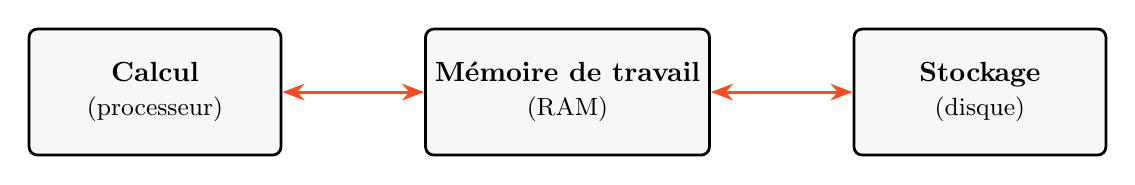
\begin{tikzpicture}[
  box/.style={draw=NouBlack,line width=1pt,rounded corners=3pt,minimum width=3.2cm,minimum height=1.6cm,align=center,fill=black!3},
  lien/.style={<->,>=Stealth,line width=1.1pt,NouOrange}]
  \node[box] (calc) {\textbf{Calcul}\\{\small (processeur)}};
  \node[box,right=1.8cm of calc] (mem) {\textbf{Mémoire de travail}\\{\small (RAM)}};
  \node[box,right=1.8cm of mem] (sto) {\textbf{Stockage}\\{\small (disque)}};
  \draw[lien] (calc) -- (mem);
  \draw[lien] (mem) -- (sto);
\end{tikzpicture}
\end{document}
